\documentclass[main.tex]{subfiles}
\begin{document}


\section{HTML}
Hypertext Markup Language je značkovací jazyk určený pro zobrazení webovým prohlížečem, používaný pro tvorbu statických webových stránek. Spolu s CSS a javascriptem patří k základním technologiím používaným při vývoji webových stránek. Tak jako i jiné zančkovací jazyky, je i HTML dokument formátován značkami, tzv. tagy, které předdefinovaným způsobem formátují dokument do výsledné podoby. Tagy jsou uzavírány do špičatých závorek $<p>$ \cite{web:wik:en:html} V součastnosti k tomu slouží kolem 110 formátovacích tagů. Neurčitost je dána rozdílnými způsoby počítání, k nimž se dostaneme v podkapitole Specifikace. \cite{web:en:countinghtml}


\subsection{Historie}
Autorem jazyka je Tim Berners-Lee, který jej vyvinul za účelem zjednodušení výroby vědeckých dokumentů, které byly psány v jazycích TeX, PostScript a SGML (Standard Generalized Markup Language). SGML se stal pro HTML předlohou. Samotné HTML publikoval Tim Berners-Lee v roce 1990, spolu s webovým protokolem HTTP (hyper text transfer protocol), sloužícím k přenosu HTML stránky po internetu. 26. února 1991 představil Berner-Lee také první webový prohlížeč, který nazval WorldWideWeb.
Verze HTML 0.9 - 1.2 vznikly v letech 1991 - 1993, avšak nepodporovaly grafické rozhraní - bylo možné zobrazovat pouze standartní znaky. Dále byla v listopadu 1995 vydána verze 2.0, ve které byla přidána podpora grafiky a interaktivních formulářů. Následovaly verze 3.0 v roce 1997, 4.0 v roce 1999. Zatím poslední verze jazyka - HTML 5.3, byla vydána 22. prosince 2022. HTML je tedy stále aktivně vyvíjeno. \cite{web:wik:en:html}


\subsection{Specifikace}
HTML je strukturováno množinou tagů, které mohou mít vlastnosti (atributy). Tag se skládá z názvu tagu uzavřeném mezi špičatými závorkami. Tagy jsou obvykle párové, přičemž počáteční značka se shoduje s koncovou. Koncová má navíc před názvem lomítko. Tag ovlivňuje veškerý obsah mezi značkami, což mohou být i další tagy. Atributy tagu se zapisují za název první značky, a dále určují vlastnosti tagu. V ukázce níže je tag, který slouží pro vytvoření odkazu. Jeho atributy jsou v tomto případě href, který udává, kam se má uživatel dostat po kliknutí na odkaz, a target, jenž definuje, že se má odkaz otevřít v novém okně prohlížeče.\cite{web:wik:en:html}
		\begin{figure}[h]
			\centering
			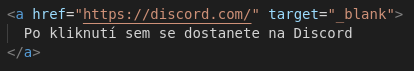
\includegraphics[width=.7\textwidth]{./html/tags.png}
			\caption{Znazornění třídy}
		\end{figure}



Nepárové tagy mají pouze jednu značku - postrádají koncovou, a nemají žádný obsah. Příkladem buď tag includegraphics, jenž do dokumentu přidá obrázek "obrazek.jpg".
		\begin{figure}[h]
			\centering
			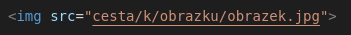
\includegraphics[width=.7\textwidth]{./html/img.png}
			\caption{Znazornění třídy}
		\end{figure}

Počet HTML tagů se v jednotlivých verzích liší. HTML 1.0 definovalo 22 značek. Jejich počet se v 3.2 zvýšil na 70, a dále v HTML 5.2 je jich definováno 111. Počítáme-li k nim i tagy XHTML specifikace, dostaneme 133. \cite{web:en:counting_html}

\end{document}

